\clearpage

\section{Исследование технологий, применяемых для построения компиляторов}

LLVM (первоначально аббревиатура расшифровывалась как Low Level Virtual Machine) начался как
исследовательский проект Университета штата Иллинойс. Целью проекта было разработать промежуточное
представление (intermediate representation, IR), основанное на SSA (single static assignment) 
форме, способное описывать конструкции высокоуровневых языков программирования, а так же
универсальный набор оптимизаций над этим представлением. Неполный список проектов, входящих
в состав LLVM, включает в себя:

\begin{enumerate}
\item Ядро библиотеки, содержащее инструменты для работы с LLVM IR, а так же набор
оптимизаций и трансформаций над ним.
\item Clang -- фронтенд для C, C++ и Objective-C.
\item LLDB -- отладчик для C, C++ и Objective-C программ.
\item libc++ -- имплементация стандартной библиотеки C++.
\item OpenMP -- библиотеки времени исполнения для поддержки стандарта OpenMP.
\item LLD -- линковщик.
\item MLIR -- Multi-Level Intermediate Representation, набор библиотек для
создания собственных высокоуровневых промежуточных представлений и трансформаций
над ними. 
\end{enumerate}

\subsection{Промежуточное представление программного кода}
Static single assignment form (SSA) -- промежуточное представление, в котором
значения переменным присваиваются лишь один раз. Используется компиляторами для
упрощения процесса оптимизации программного кода. Изменяемость переменных может
достигаться двумя путями. Первый -- выделять динамическую память и обновлять
значения операциями чтения и записи в память (\textit{load and store}). Этот
метод использует clang. Однако в таком виде затрудняется статический анализ
памяти (dataflow analysis). Более удобным способом будет добавление суффикса к
имени переменной. В некоторых случаях первая форма может быть приведена ко 
второй с помощью процедуры под названием \textit{memory to register}.
% https://ru.wikipedia.org/wiki/SSA

\subsection{Технологии компиляции исходного кода <<на лету>>}
Компиляция <<на лету>> (англ. \textit{Just-in-time compilation, JIT}) --
один из видов компиляции, когда промежуточное представление программы, 
называемое байт-код, преобразуется в машинные инструкции прямо во время
исполнения программы. В отличие от компиляции перед выполнением (англ. 
\textit{Ahead-of-time compilation, AOT}), JIT позволяет оптимизировать код
программы непосредственно под архитектуру платформы, на которой программа
исполняется, за счет чего достигается повышение производительности. Однако, у
JIT есть недостаток -- увеличенное время запуска программы. В случае, если она
не выполняет сложных вычислений, время запуска и компиляции может превысить 
время работы.
% https://ru.wikipedia.org/wiki/JIT-%D0%BA%D0%BE%D0%BC%D0%BF%D0%B8%D0%BB%D1%8F%D1%86%D0%B8%D1%8F
\subsubsection{Компиляция на основе технологии ORC JIT}
Одна из реализаций JIT компилятора в LLVM носит название ORC (On Request 
Compiler). ORC предоставляет модульный набор программных интерфейсов для 
построения собственных компиляторов. Среди его возможностей:
\begin{enumerate}
\item \textbf{JIT-компоновка} позволяет линковать релоцируемые объекты во время
исполнения программы.
\item \textbf{Компиляция LLVM IR} непосредственно в машинный код.
\item \textbf{Упереждающая и <<ленивая>> компиляция} (англ. \textit{eager and
lazy compilation}). В первом случае вся программа компилируется непосредственно
перед запуском программы и сохраняется в оперативной памяти. Во втором случае
код каждой процедуры компилируется непосредственно перед её вызовом.
\item \textbf{Многопоточная компиляция}.
\end{enumerate}
% https://llvm.org/docs/ORCv2.html

\subsection{Оптимизации программного кода во время компоновки}
Компоновщик -- специальная программа, производящая компоновку (линковку, англ.
\textit{linking}), т.е. связывание бинарных модулей в исполняемый файл.
% https://ru.wikipedia.org/wiki/%D0%9A%D0%BE%D0%BC%D0%BF%D0%BE%D0%BD%D0%BE%D0%B2%D1%89%D0%B8%D0%BA
\subsubsection{Оптимизации с применением технологии ThinLTO}
Оптимизация во время компоновки (англ. \textit{Link time optimization}) -- один
из методов, позволяющий достигать лучшей производительности путем анализа целой
программы (в противоположность классическому анализу единиц трансляции) и
кросс-модульной оптимизации. Во время компиляции вместо машинного кода выдается
промежуточное представление программы, над которым линковщик может совершать
манипуляции.

ThinLTO -- новый подход в LLVM для подобных оптимизаций, впервые представленный
компанией Google в 2015 году\cite{Johnson}.

Процесс компиляции с ThinLTO разделен на 3 фазы:
\begin{enumerate}
  \item \textbf{Компиляция}. Генерация промежуточного представления как полного
        LTO модуля, но дополненного кратким содержанием модулей.
  \item \textbf{Легкая компоновка}. Соединение всех кратких содержаний в единое
        и проведение глобального анализа.
  \item \textbf{ThinLTO backend}. Многопоточные оптимизации с использованием
        данных, полученных на предыдущем шаге.
\end{enumerate}
\begin{figure}[h]
  \centering
  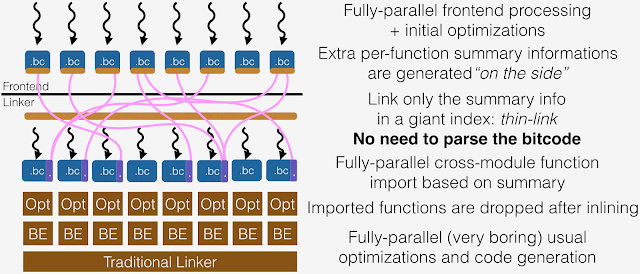
\includegraphics[width=\textwidth]{thinlto.png}
  \caption{ThinLTO. Источник: \url{http://blog.llvm.org/2016/06/thinlto-scalable-and-incremental-lto.html}}
\end{figure}
% https://clang.llvm.org/docs/ThinLTO.html
% http://blog.llvm.org/2016/06/thinlto-scalable-and-incremental-lto.html

\subsection{Исследование инструментов трансляции исходного кода в промежуточное представление}
Проект Clang предоставляет фронтэнд и инфраструктуру для построения инструментов
для работы с C-подобными языками программирования (C, C++, Objective-C,
OpenCL C, CUDA, RenderScript) для LLVM. Благодаря модульной архитектуре, Clang
может выступать не только как компилятор, но и как средство статического анализа
кода, утилита автоматического форматирования, языковой сервер и т.д.

\begin{figure}[h]
  \centering
  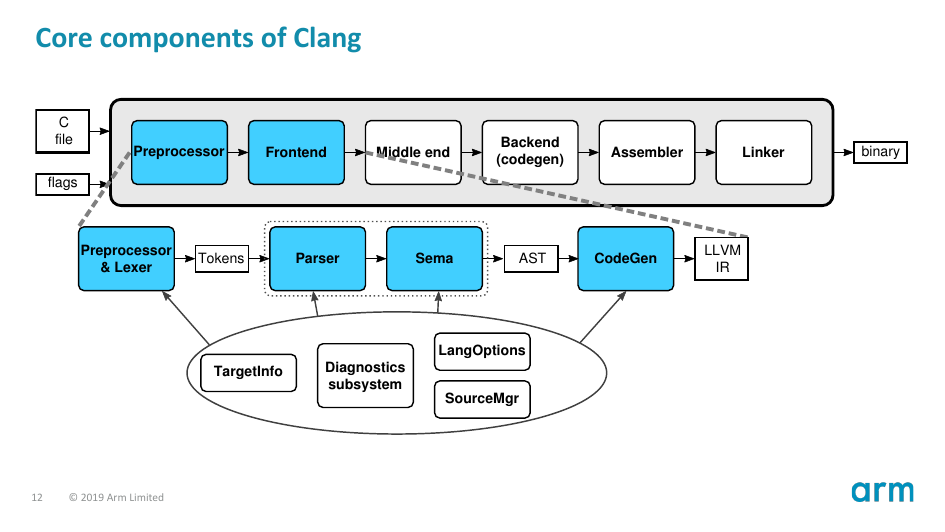
\includegraphics[width=\textwidth]{clangTutorial-18}
  \caption{Ключевые компоненты Clang. Источник: \cite{VanHaagstretSvenARMandStulova2019}}
  \label{fig:clang_core}
\end{figure}
% https://www.youtube.com/watch?v=5kkMpJpIGYU
% http://llvm.org/devmtg/2019-10/talk-abstracts.html#tut8
\subsubsection{Драйвер компилятора и интерфейс командной строки}
Интерфейсом взаимодействия между пользователем и компилятором является драйвер.
Clang предоставляет GCC- и MSVC-совместимые драйверы. Задача драйвера --
распознать аргументы командной строки и сформировать последовательность действий,
которые необходимы для выполнения команды. Основная работа Clang заключается
в выполнении следующей последовательности шагов: чтение файла с исходным текстом,
препроцессинг, разбиение на ключевые слова (англ. \textit{tokens}), лексический
анализ, семантический анализ, генерация абстрактного синтаксического дерева,
генерация LLVM IR (см. рис. \ref{fig:clang_core}).

\subsubsection{Абстрактное синтаксическое дерево}
Абстрактное синтаксическое дерево (англ. \textit{Abstract Syntax Tree, AST}) --
направленный ациклический граф, вершинами которого являются конструкции языка 
программирования (декларации, циклы, операции), а ребрами -- зависимости между
ними. В AST входят не только <<видимые>> конструкции языка, но и служебные,
например, неявное преобразование типов. Это делает подобные деревья хорошей
базой для генерации промежуточного представления. Кроме того, Clang позволяет
превращать AST обратно в исходный код, что позволяет строить на его основе
различные инструменты автоматизации разработки.
\begin{figure}[h]
  \centering
  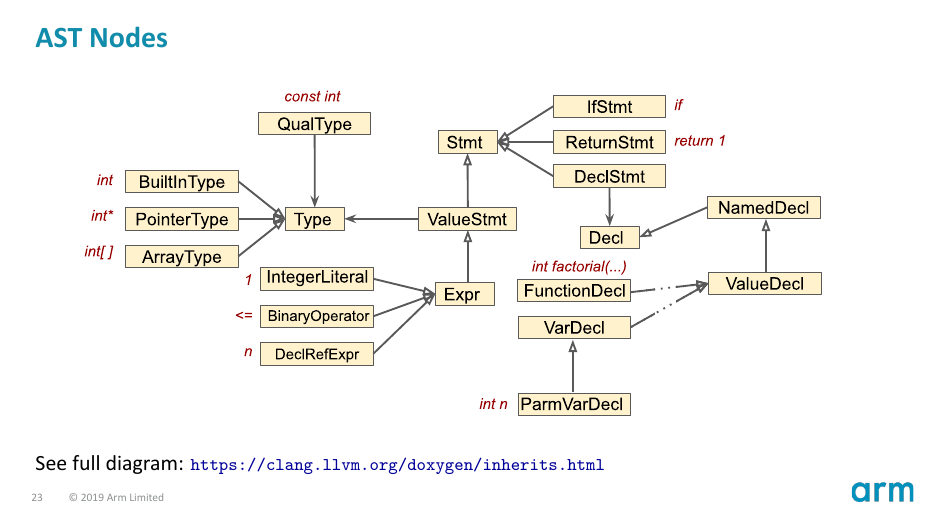
\includegraphics[width=\textwidth]{clangTutorial-48}
  \caption{Основные классы Clang AST. Источник: \cite{VanHaagstretSvenARMandStulova2019}}
  \label{fig:clang_core}
\end{figure}

Ниже представлен исходный код на языке C.
\lstinputlisting[language=C,caption={Пример программы на языке C}]{listings/factorial.c}
Текстовое представление AST для этого фрагмента кода можно увидеть в листинге
\ref{lst:clang_ast} Приложения. На рис. \ref{fig:clang_ast} можно увидеть
графическое представление данного дерева.

\begin{figure}[h]
  \centering
  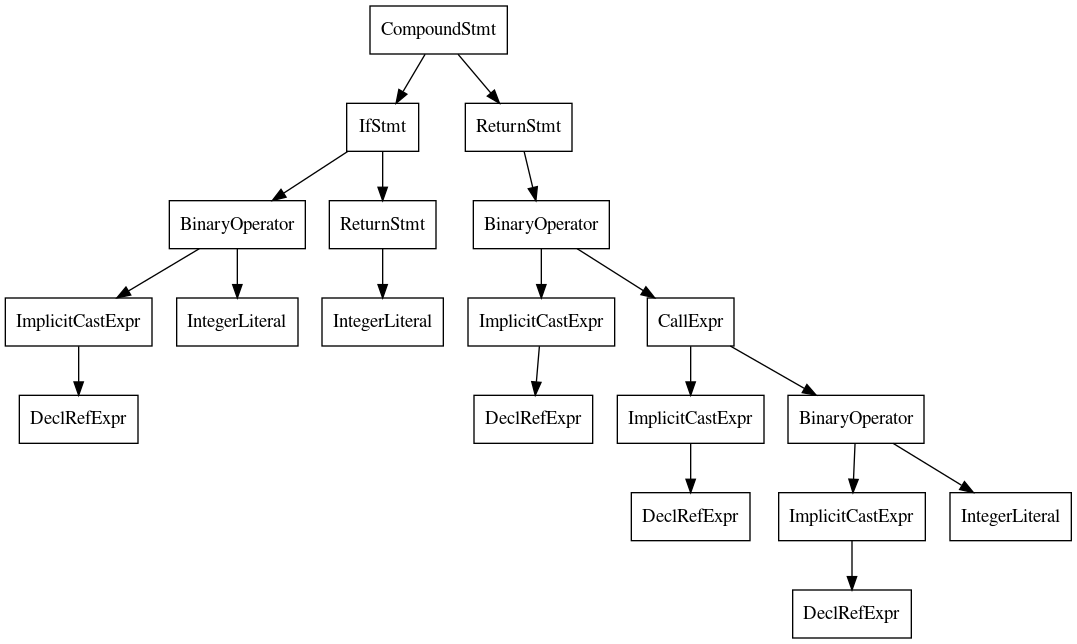
\includegraphics[width=\textwidth]{ast_factorial}
  \caption{Графическое представление Clang AST} 
  \label{fig:clang_ast}
\end{figure}

% TODO example of C function, AST, and AST Graph

\subsubsection{Генерация промежуточного представления из абстрактного синтаксического дерева}
Когда получен AST, компилятор может приступать к генерации кода. В случае с LLVM
перед генерацией машинных инструкций строится описанное ранее промежуточное
представление. Для получения LLVM IR из синтаксического дерева Clang использует
алгоритм обхода графа в глубину. Пример полученного IR можно увидеть в листинге
\ref{lst:llvm_ir_clang} Приложения.

\subsection{Многоуровневое промежуточное представление}
MLIR -- это новая инфраструктура для разработки промежуточных представлений.
По заверениям авторов, ее задача -- борьба с фрагментацией программного
обеспечения, улучшения качества гетерогенной компиляции, уменьшение стоимости
разработки новых компиляторов. MLIR предоставляет инструменты для создания
генераторов кода, трансляторов, оптимизаторов на разных уровнях абстракции\cite{Lattner2020}.
% https://mlir.llvm.org/
% http://llvm.org/devmtg/2019-04/talks.html#Keynote_1
\subsubsection{Диалекты}
Основная идея в MLIR заключается в том, что для разных задач требуется разный
уровень абстракций. В процессе преобразования исходного кода в LLVM IR теряется
информация о конструкциях языка, которая могла бы быть использована для
оптимизации программы. С похожими трудностями сталкиваются разработчики
фреймворков для машинного обучения: в процессе преобразования теряются знания
о предметной области. Основной единицей в MLIR является <<Диалект>> -- набор
типов данных и операций над ними. С помощью диалекта можно описать предметную
область и задать преобразования над этими данными. Кроме того, доступны
механизмы преобразования из одного диалекта в другой. Это позволяет
переиспользовать уже имеющиеся инструменты, переходя от более высокого уровня
абстракции к более низким, когда оптимизации на текущем уровне более невозможны.
Такой стратегии, например, придерживается Tensorflow (рис. \ref{fig:tf_dialects}).
% https://www.youtube.com/watch?v=ff3ngdvUang&feature=youtu.be
\begin{figure}[h]
    \centering
    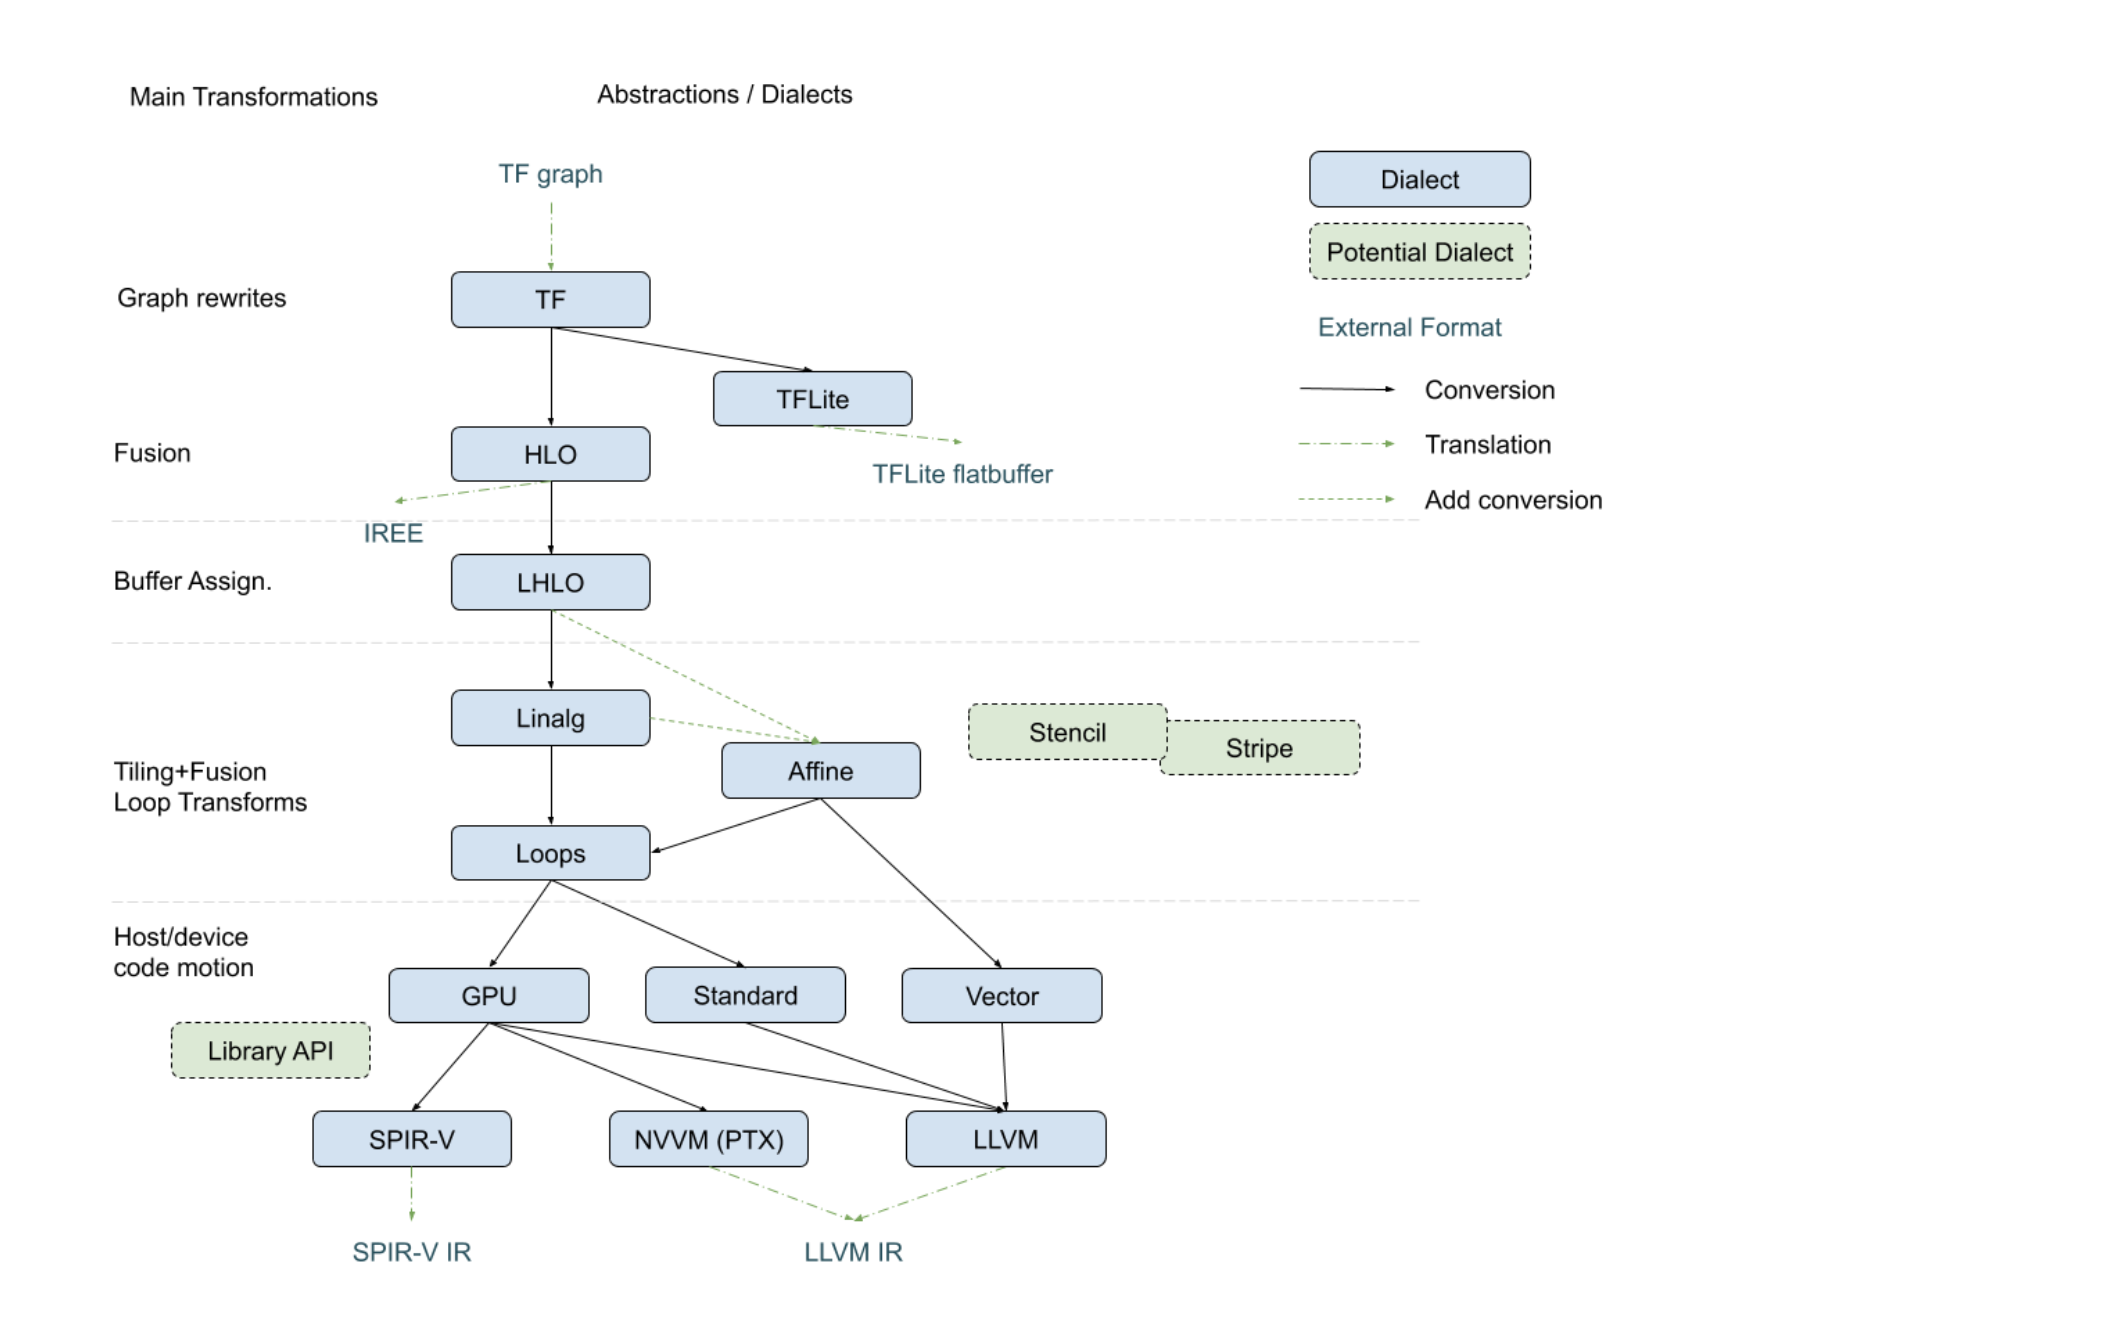
\includegraphics[width=\textwidth]{mlir_vector_dialect.png}
    \caption{Пример взаимодействия диалектов. Источник: \url{https://bit.ly/2YdmVhf}
   % https://docs.google.com/presentation/d/1P-j1GrH6Q5gLBjao0afQ-GfvcAeF-QU4GXXeSy0eJ9I/edit#slide=id.p
    }
    \label{fig:tf_dialects}
\end{figure}
\subsubsection{Упрощенное полиэдральное представление}
Одна из основных конструкций классических языков программирования -- циклы.
Возможность исполнять один и тот же код много раз -- важный инструмент обработки
данных. Его можно сделать еще более гибким, если ввести новую абстракцию и
представить вложенные циклы как аффинное пространство. Любая комбинация
индексных переменных будет точкой в этом пространстве, а множество всех таких
точек -- полиэдром. Используя подобную абстракцию, можно свести оптимизацию
вложенных циклов к аффинным преобразованиям. MLIR предоставляет упрощенное
представление подобных конструкций путем введения в грамматику промежуточного
представления размерностей (англ. \textit{dimensions}) -- идентификаторов,
соответствующих размерности представляемой структуры (т.е. циклов), и символов --
произвольных числовых констант неизвестного происхождения\footnote{\url{https://mlir.llvm.org/docs/Dialects/Affine/}}.
Используя эти данные, фреймворк может выполнять <<склеивание>>,
<<разворачивание>>, векторизацию циклов.
